\documentclass[10pt,times]{beamer}
\usepackage{amsfonts}
\usepackage{amsmath}
\usepackage{amssymb}
\usepackage{mathptmx}

\usepackage{color}
\usepackage{minted}
\usepackage{hyperref}
\usepackage{multicol}
\usepackage{tabularx}
\usepackage{booktabs}
\usepackage{menukeys}

% Stolen from John Miller's LaTeX course
\newcommand{\bftt}[1]{\textbf{\texttt{#1}}}
\newcommand{\comment}[1]{{\color[HTML]{008080}\textit{\textbf{\texttt{#1}}}}}
\newcommand{\cmmd}[1]{{\color[HTML]{008000}\bftt{#1}}}
\newcommand{\bs}{$\backslash$}
\newcommand{\cmdbs}[1]{\cmmd{\bs#1}}
\newcommand{\lb}{{\char'173}}% Left brackets -> {
\newcommand{\rb}{{\char'175}}% Right brackets -> }
\newcommand{\cmdbegin}[1]{\cmdbs{begin\lb}\bftt{#1}\cmmd{\rb}}
\newcommand{\cmdend}[1]{\cmdbs{end\lb}\bftt{#1}\cmmd{\rb}}



% this is where the example source files are loaded from
% do not include a trailing slash
\newcommand{\wllogo}{\textbf{Overleaf}}
\newcommand{\fileuri}{https://raw.githubusercontent.com/kks32/latex-course/master/exercises/}
\newcommand{\wlserver}{https://www.overleaf.com}
\newcommand{\wlnewdoc}[1]{\wlserver/docs?snip\_uri=\fileuri#1\&splash=none}

\def\tikzname{Ti\emph{k}Z}


% stolen from minted.dtx
\newenvironment{exampletwoup}
  {\VerbatimEnvironment
   \begin{VerbatimOut}{example.out}}
  {\end{VerbatimOut}
   \setlength{\parindent}{0pt}
   \fbox{\begin{tabular}{l| l}
   \begin{minipage}{0.55\linewidth}
     \inputminted[fontsize=\small,resetmargins]{latex}{example.out}
   \end{minipage} &
   \begin{minipage}{0.35\linewidth}
     \input{example.out}
   \end{minipage}
   \end{tabular}}}

\newenvironment{exampletwouptiny}
  {\VerbatimEnvironment
   \begin{VerbatimOut}{example.out}}
  {\end{VerbatimOut}
   \setlength{\parindent}{0pt}
   \fbox{\begin{tabular}{l|l}
   \begin{minipage}{0.55\linewidth}
     \inputminted[fontsize=\scriptsize,resetmargins]{latex}{example.out}
   \end{minipage} &
   \begin{minipage}{0.35\linewidth}
     \setlength{\parskip}{6pt plus 1pt minus 1pt}%
     \raggedright\scriptsize\input{example.out}
   \end{minipage}
   \end{tabular}}}

% ******************************** Meta-data ***********************************
\mode<presentation>
{
  \usetheme{Madrid}
  \setbeamercovered{transparent}
}


\usepackage{caption}
\captionsetup{font=scriptsize, labelfont=scriptsize, justification=centering}

\title{Writing papers and thesis using \LaTeX2e}

\author {Krishna Kumar \inst{*}\thanks{kks32@cam.ac.uk} }

\institute[ University of Cambridge ] % (optional, but mostly needed)
{
  \inst{1}%
  King's College\\
  University of Cambridge
}

\date[LaTeX course 2014] % (optional, should be abbreviation of conference name)
{\LaTeX for Beginners}


% Delete this, if you do not want the table of contents to pop up at
% the beginning of each subsection:
%\AtBeginSubsection[]
%{
%  \begin{frame}<beamer>{Outline}
%    \tableofcontents[currentsection,currentsubsection]
%  \end{frame}
%}


% If you wish to uncover everything in a step-wise fashion, uncomment
% the following command: 

% \beamerdefaultoverlayspecification{<+->}

\subtitle{Part I: Writing papers using \LaTeX}
%***************************** Title page **************************************
\begin{document}
\begin{frame}
  \titlepage
\end{frame}
%*******************************************************************************
%**************************** Introduction *************************************
%*******************************************************************************
\section{Sections and subsections}

%*******************************************************************************
%******************************* Frame *****************************************
%*******************************************************************************
\begin{frame}{Sections}
\begin{itemize}
\item To generate sections in \LaTeX: \cmdbs{section\{name-here\}}
\item Subsection: \cmdbs{subsection\{name-here\}}
\item Subsubsection: \cmdbs{subsubsection\{name-here\}}
\item Subsections without numbering \cmdbs{subsection*\{name-here\}}

\end{itemize}
\end{frame}



%*******************************************************************************
%******************************* Frame *****************************************
%*******************************************************************************
\subsection{Sections}
\begin{frame}{\insertsubsection}
\begin{minipage}{0.55\linewidth}
\inputminted[fontsize=\scriptsize,frame=single,resetmargins]{latex}%
  {structure-sections.tex}
\end{minipage}
\begin{minipage}{0.35\linewidth}
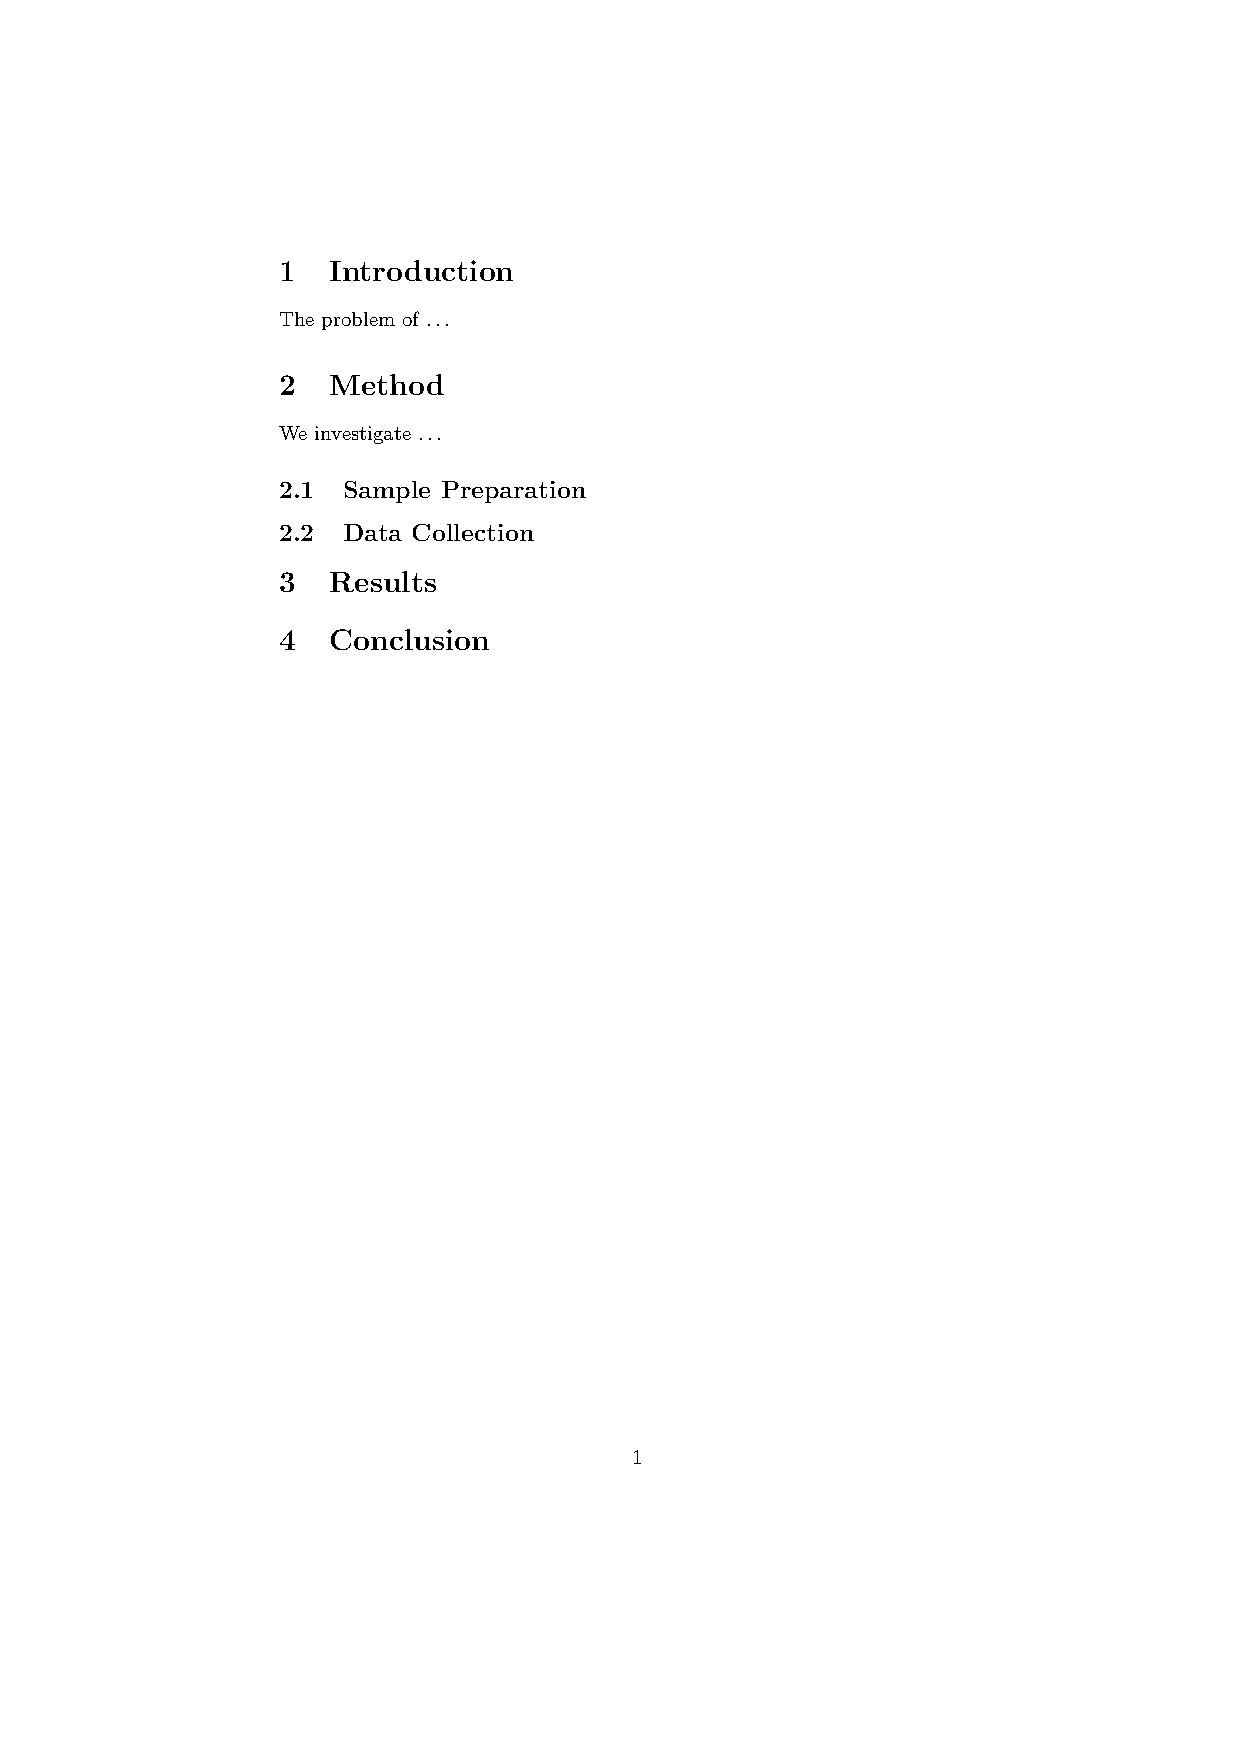
\includegraphics[width=\textwidth,clip,trim=1.5in 6in 4in 
1in]{structure-sections.pdf}
\end{minipage}
\end{frame}

%*******************************************************************************
%******************************* Frame *****************************************
%*******************************************************************************
\subsection{Title and abstract}
\begin{frame}{Title and Abstract}
Before you begin typing your document, i.e., \cmdbs{begin\{document\}} you need 
to define the author name and title.
\begin{itemize}
\item Title of the document in \LaTeX: \cmdbs{title\{name-here\}}
\item Author name: \cmdbs{author\{name-here\}}
\item Set a specific date: \cmdbs{date\{date-here\}}
\item How do you not print date: \cmdbs{date\{\}}
\end{itemize}
\centering
This only defines what the title of the document, author name and date create. 
It does not print it. To print the meta-data, do \cmdbs{maketitle} after begin 
document
\end{frame}

%*******************************************************************************
%******************************* Frame *****************************************
%*******************************************************************************

\subsection{Title and Abstract}
\begin{frame}[fragile]{\insertsubsection}
\begin{itemize}{\small
\item Tell \LaTeX{} the \cmdbs{title} and \cmdbs{author} names in the preamble.
\item Then use \cmdbs{maketitle} in the document to actually create the title.
\item Use the \bftt{abstract} environment to make an abstract.
}\end{itemize}
\centering
\begin{minipage}{0.45\linewidth}
\inputminted[fontsize=\scriptsize,frame=single,resetmargins]{latex}%
  {structure-title.tex}
\end{minipage}
\begin{minipage}{0.45\linewidth}
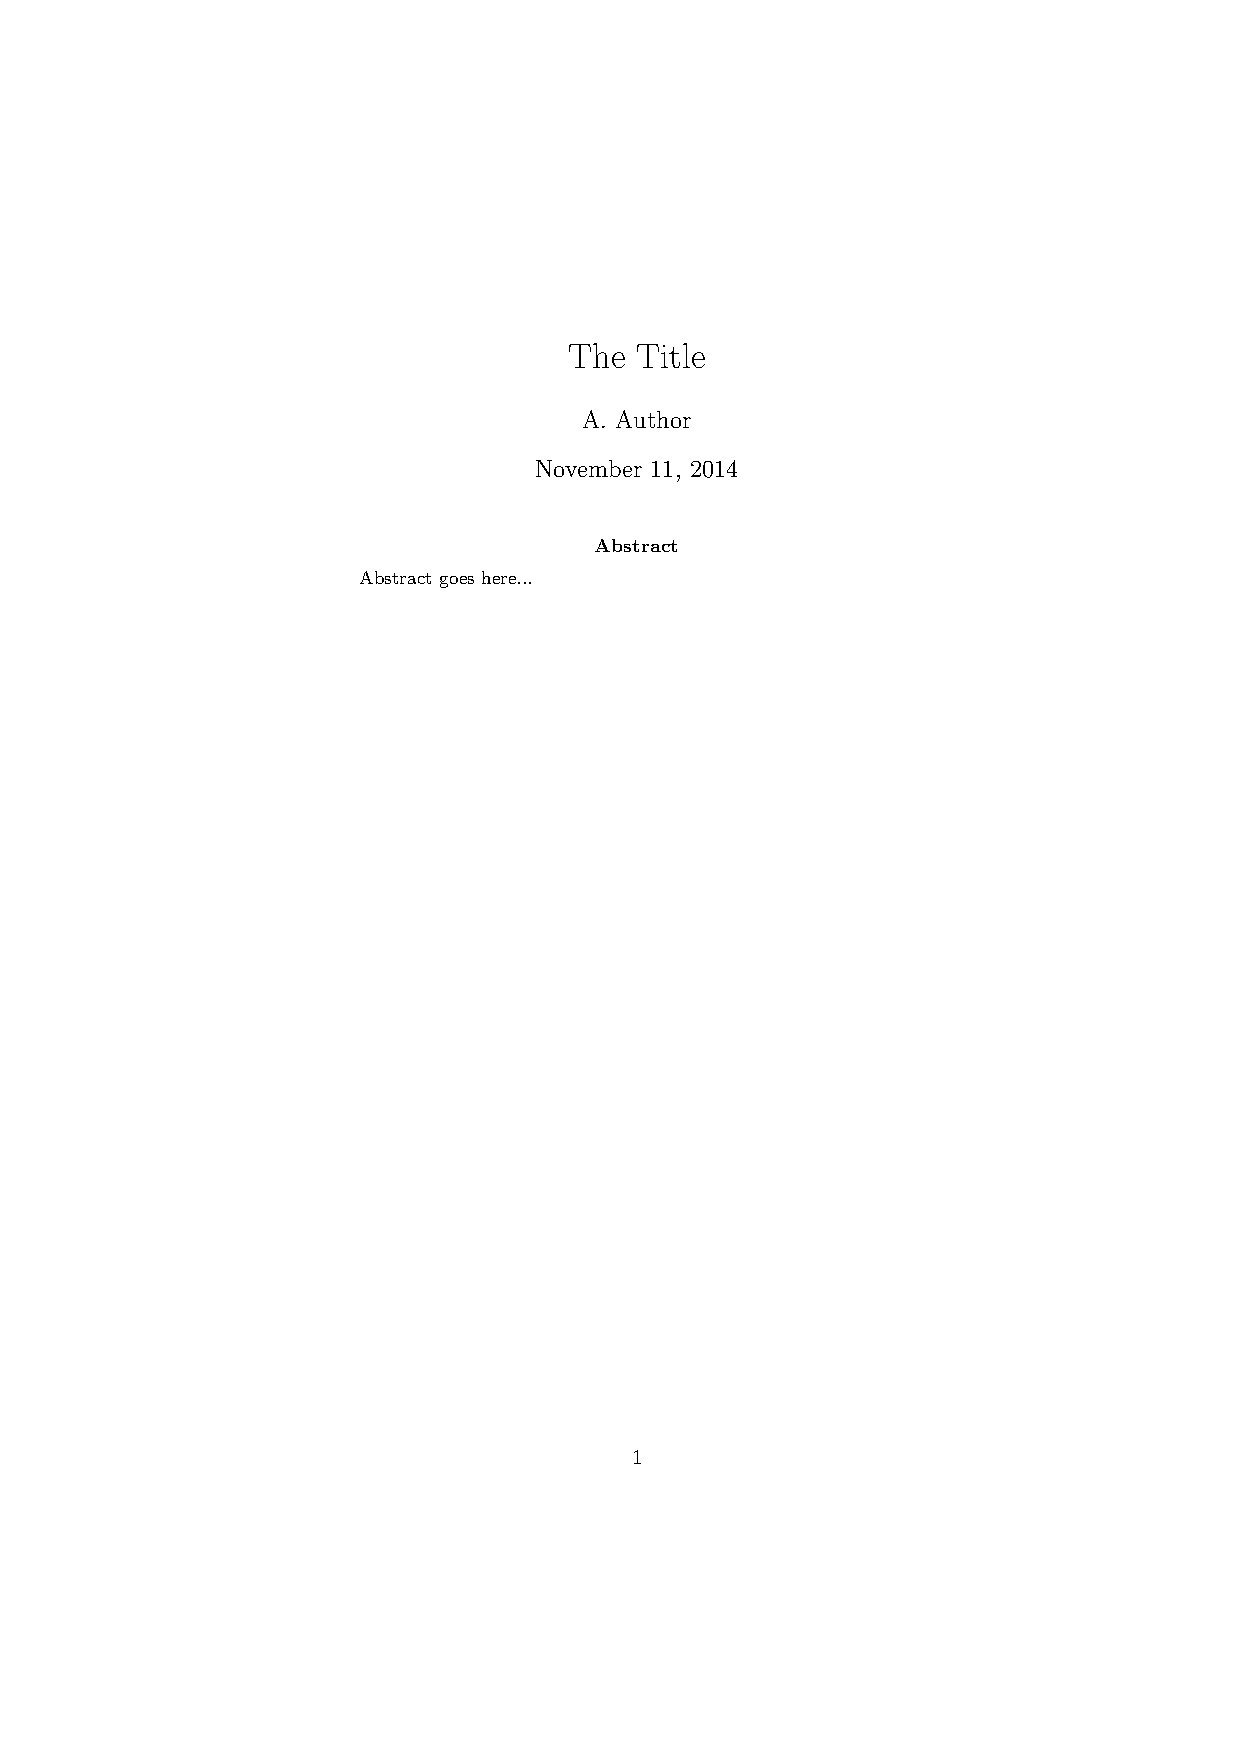
\includegraphics[width=\textwidth,clip,trim=2.2in 7in 2.2in 
2in]{structure-title.pdf}
\end{minipage}
\end{frame}

%*******************************************************************************
%******************************* Frame *****************************************
%*******************************************************************************

\begin{frame}{\bs documentclass$[$\textbf{options}$]$\{\}}
\begin{table}
\renewcommand{\arraystretch}{1.2}
\begin{tabularx}{0.97\textwidth}{lll}
\toprule
\textbf{Argument} & \textbf{Possible Values} & \textbf{Default Value} \\
\midrule
Typeface Size & 10pt, 11pt, 12pt & 10pt   \\
Paper Size & a4paper, a5paper, & letterpaper \\
				& letterpaper, legalpaper &  \\
				& executivepaper b5paper &  \\
Paper Orientation & portrait, landscape & portrait \\
Title Page & titlepage, notitlepage & titlepage \\
Equation Numbering & leqno & Right side \\ 
Equation Alignment & fleqn & Centered \\ 
Output Type				& draft, final & final \\
Layout Type & oneside, twoside & oneside  \\
Chapter Opening & openright, openany & openright \\
Columns & onecolumn, twocolumn & onecolumn \\
\bottomrule
\end{tabularx}
\end{table}
\end{frame}


%*******************************************************************************
%******************************* Frame *****************************************
%*******************************************************************************
\begin{frame}{Font types}
\begin{block}{Font face}
\bs emph\{\emph{text}\}, 
\bs textbf\{\textbf{text}\}, 
\bs textit\{\textit{text}\},
\bs texttt\{\texttt{text}\},
\bs textrm\{\textrm{text (roman)}\},
\bs textsf\{\textsf{text (sans font)}\},
\bs textsc\{\textsc{text}\}
\end{block}
\begin{block}{Font size}
\tiny \bs tiny,
\scriptsize \bs scriptsize,
\footnotesize \bs footnotesize,
\small \bs small,
\normalsize \bs normalsize,
\large \bs large,
\Large \bs Large,
\LARGE \bs LARGE,
\huge \bs huge,
\Huge \bs Huge
\end{block}

\begin{block}{Alignment}
\cmdbegin{flushleft / flushright / center}\\
\ldots\\
\cmdend{flushleft / flushright / center}
\end{block}
\end{frame}

%*******************************************************************************
%******************************* Frame *****************************************
%*******************************************************************************
\begin{frame}{Exercise 4: Sections}
\begin{itemize}
\item Add title, author and print date
\item Set font size to 11 pt
\item Create sections and subsections
\end{itemize}
\begin{center}
\fbox{\href{\wlnewdoc{Ex4-Sections/Ex4-Sections.tex}}{%
Click to open this exercise in \wllogo{}}}
\end{center}

\begin{itemize}
\item Hint: Don't forget to do \cmdbs{maketitle} and don't forget 
\cmmd{begin\{document\}} and \cmmd{end\{document\}}
\fbox{\href{\wlnewdoc{Ex4-Sections/Ex4-Sections-solution.tex}}{%
click here to see my solution}}.
\end{itemize}

\end{frame}


%*******************************************************************************
%******************************* Frame *****************************************
%*******************************************************************************
\section{Maths}
\begin{frame}[fragile]{Typesetting Maths}
\begin{itemize}
\item Why are dollar signs \keys{\$} special? We use them to mark mathematics 
in text.\\[1ex]
\begin{exampletwouptiny}
% not so good:
Let a and b be distinct positive
integers, and let c = a - b + 1.

% much better:
Let $a$ and $b$ be distinct positive
integers, and let $c = a - b + 1$.
\end{exampletwouptiny}
\item Always use dollar signs in pairs --- one to begin the mathematics, and one
to end it.
\item \LaTeX{} handles spacing automatically; it ignores your spaces.
\begin{exampletwouptiny}
Let $y=mx+b$ be \ldots

Let $y = m x + b$ be \ldots
\end{exampletwouptiny}

\end{itemize}
\end{frame}


%*******************************************************************************
%******************************* Frame *****************************************
%*******************************************************************************
\begin{frame}[fragile]{Notation}
\begin{itemize}
\item Use caret \verb|^| for superscripts and underscore \cmmd{`\_'} 
for subscripts.
\begin{exampletwouptiny}
$y = c_2 x^2 + c_1 x + c_0$
\end{exampletwouptiny}
\vskip 2ex

\item Use curly braces $\{$ and $\}$ to group
superscripts and subscripts.
\begin{exampletwouptiny}
$F_n = F_n-1 + F_n-2$     % oops!

$F_n = F_{n-1} + F_{n-2}$ % ok!
\end{exampletwouptiny}
\vskip 2ex

\item There are commands for Greek letters and common notation.
\begin{exampletwouptiny}
$\mu = A e^{Q/RT}$

$\Omega = \sum_{k=1}^{n} \omega_k$
\end{exampletwouptiny}
\end{itemize}
\end{frame}

%*******************************************************************************
%******************************* Frame *****************************************
%*******************************************************************************
\begin{frame}[fragile]{Inline equations}
\begin{itemize}
\item If it's big and scary, \emph{display} it on its own line using
\cmdbegin{equation} and \cmdend{equation}.\\[2ex]
\begin{exampletwouptiny}
The roots of a quadratic equation
are given by
\begin{equation}
x = \frac{-b \pm \sqrt{b^2 - 4ac}}{2a} \,.
\end{equation}
where $a$, $b$ and $c$ are \ldots
\end{exampletwouptiny}
\vskip 1em
{\scriptsize Caution: \LaTeX{} mostly ignores your spaces in mathematics, but it
can't handle blank lines in equations --- don't put blank lines in your
mathematics.}
\item You can add punctuations in your equation by adding \cmdbs{,.} to add a 
period and \cmdbs{,,} to add a comma at the end of the equation.
\end{itemize}
\end{frame}


%*******************************************************************************
%******************************* Frame *****************************************
%*******************************************************************************
\begin{frame}{Ex 5a: Maths}

\begin{itemize}
\item Make sure inline equations are within the mathmode \cmmd{\$\dots\$}
\item Format these two equations:
\begin{equation*}
i \hbar \frac{\partial}{\partial t} \Psi(r,t) = 
\left[\frac{-\hbar^2}{2\mu}\nabla^2+V(r,t)\right]\Psi(r,t) \,,
\end{equation*}

\begin{equation*}
E^2 = (pc)^2 + (m_0 c^2)^2 \,.
\end{equation*}

\begin{center}
\fbox{\href{\wlnewdoc{Ex5-Math/Ex5-Math.tex}}{%
Click to open this exercise in \wllogo{}}}
\end{center}
\item To format math you need to use \cmmd{equation} environment
\item Use detexify to find out what the symbols are 
\href{http://detexify.kirelabs.org/classify.html}{http://detexify.kirelabs.org/classify.html}
\fbox{\href{\wlnewdoc{Ex5-Math/Ex5-Math-solution.tex}}{%
click here to see my solution}}.
\end{itemize}

\end{frame}


%*******************************************************************************
%******************************* Frame *****************************************
%*******************************************************************************
\begin{frame}{Ex 5b: Maths}

\begin{itemize}
\item Align equations as shown below:

\begin{align}
	y   & =  ax+b \nonumber\\
	y+1 & = ax+(b+1)\\
	    & = ax+(b+2)-1
\end{align}

\begin{align}
\label{eq:yequation}
\begin{aligned}
	y   & =  ax+b \\
	y+1 & = ax+(b+1)\\
	    & = ax+(b+2)-1
\end{aligned}
\end{align}

\begin{center}
\fbox{\href{\wlnewdoc{Ex5-Math/Ex5-Math.tex}}{%
Click to open this exercise in \wllogo{}}}
\end{center}
\item Insert cross references use \cmdbs{usepackage\{cleveref\}}.
\item Use \cmmd{align} environment. To use this environment you need include 
\cmdbs{usepackage\{amsmath\}} and \cmdbs{usepackage\{amsfonts\}} packages.
\end{itemize}
\begin{center}
\fbox{\href{\wlnewdoc{Ex5-Math/Ex5-Math-solution.tex}}{%
click here to see my solution}}
\end{center}
\end{frame}


%*******************************************************************************
%******************************* Frame *****************************************
%*******************************************************************************
\begin{frame}[fragile]{Never use equation arrays}
\begin{itemize}
\item Use \cmmd{align} instead of \cmmd{eqnarray} when you have multiple 
equations.
\end{itemize}
\begin{exampletwoup}
\begin{eqnarray}
E& = & m_0 c^2 \,,\\
E^2& = &(m_0 c^2)^2 + (pc)^2 \,.
\end{eqnarray}
\end{exampletwoup}
\vskip 2ex
\begin{exampletwoup}
\begin{equation}
E = m_0 c^2 \,,
\end{equation}
\begin{equation}
E^2 = (m_0 c^2)^2 + (pc)^2 \,.
\end{equation}
\end{exampletwoup}
\vskip 2ex
\begin{exampletwoup}
\begin{align}
E  =  m_0 c^2 \,,\\
E^2  = (m_0 c^2)^2 + (pc)^2 \,.
\end{align}
\end{exampletwoup}
\end{frame}

\end{document}
